\documentclass[a4paper]{scrartcl}
\usepackage[utf8]{inputenc}
\usepackage[english]{babel}
\usepackage{graphicx}
\usepackage{lastpage}
\usepackage{pgf}
\usepackage{wrapfig}
\usepackage{fancyvrb}
\usepackage{fancyhdr}
\usepackage{listings}
\pagestyle{fancy}
\usepackage{libertine}
\renewcommand*\familydefault{\sfdefault}  %% Only if the base font of the document is to be sans serif
\usepackage[T1]{fontenc}
\usepackage{courier}
\usepackage[parfill]{parskip}

\graphicspath{ {./images/} }

% Create header and footer
\headheight 27pt
\pagestyle{fancyplain}
\lhead{\footnotesize{Internet Applications, ID1354}}
\chead{\footnotesize{Assignment 2: JavaScript}}
\rhead{}
\lfoot{}
\cfoot{\thepage\ (\pageref{LastPage})}
\rfoot{}

% Create title page
\title{Assignment 2: JavaScript}
\subtitle{Internet Applications, ID1354}
\author{Emil Tullstedt [emiltu@kth.se]}
\date{2014-09-24}

\lstset{
	basicstyle=\footnotesize\ttfamily, 
	numbers=left,
	breaklines=true,
	frame=l,
	keywordstyle=\bfseries\color{blue!40!black},
    stringstyle=\color{red},
    commentstyle=\color{green},
    identifierstyle=\color{black},
    showstringspaces=false
}

\begin{document}

\maketitle

\section{Introduction}

The second assignment for ID1354 is about adding JavaScript functionality to a static web site. The task was to develop the following on the website developed for the first assignment:

\begin{itemize}
\item Create a JavaScript-powered drop-down menu
\item Develop a volatile comment field
\item Make the comments editable and delete-able
\item Add two pages containing static information
\end{itemize}

\section{Method}

\subsection{JavaScript Best Practices}

There are very few programming languages that doesn't need sensible code standards which can be controlled against using a linter. Idiomatic JavaScript is especially hard, as the programming language by default doesn't enforce either it's end-of-line character (the interpreter has to make a guess at where one line of code ends and another one begins) or variable declaration. As the language further isn't safe and has side-effects (this is a property of most imperative languages). JavaScript also has a tendency to silently die, and as the language is written to be non-blocking - might run certain functions ahead of plausible time.

Because of the \textit{flexibility} that JavaScript inherits from this design choice, the language is very prone to software bugs. This has caused several off-spring versions of JavaScript to be developed, but as the language's most important factor is the portability, neither of these versions has ever gained the same momentum as the language itself.

The JSLint tool available to check for JavaScript best-practices at \texttt{jslint.com} is rather strict because of all this. To make the check more suitable for the needs of this assignment, the following comment is inserted at the top of the JavaScript documents that are run through the lint:

\texttt{/*jslint browser: true, vars: true, white: true, indent: 4, maxlen: 80 */}

This silences "bad" placement of variables (i.e. multiple declarations within a single block [there are sensible reasons why you wouldn't want this, but neither are applicable for our case]), "bad" whitespace usage (libraries shouldn't silence this, but whitespace isn't important in JavaScript and can be safely ignored) and assumes the client is a browser. We further suggest an indentation level of 4 spaces (which, as the whitespace error is ignored, is quite unnecessary) and a maximum length of a single line in the document of 80 characters.

You also need to inform JSLint about the global variables, where the JQuery '\$'-variable is the most notable.

Furthermore, because of the issues that the design choices of JavaScript implicates, there is a syntax that allows developer to ask the browser to crash earlier when parsing what looks like invalid JavaScript. This is done by putting \texttt{"use strict";} at the top of either a JavaScript document or a function. The JSLint.com website complains about the use of the "use strict"; in top of the document and proposes you to put it at the top of the functions\footnote{You can do this by enclosing the entire document in an anonymous function - but for this purpose, that just makes the code uglier.} instead, but that is acceptable for non-reusable libraries.

\section{Result}
\label{sec:results}

\begin{figure}[!h]
  \begin{center}
    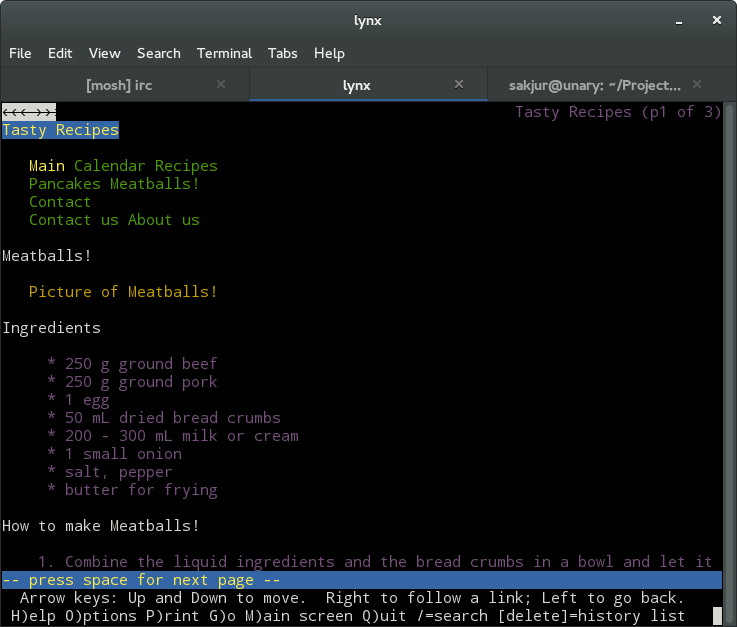
\includegraphics[scale=0.3]{lynxjavascript.png}
    \caption{The new version of the site works in Lynx}
    \label{fig:lynxjs}
  \end{center}
\end{figure}

When developing the JavaScript-version of the site, Knockout.js and other MVC implementations of JavaScript was ignored due to the fact that it is hard to develop working structures using the framework that is also accessible for all users. This caused a slight fracture to the encapsulation of the JavaScript code, but as seen in figure \ref{fig:lynxjs} assists in not breaking the site for very simple browsers.

\subsection{Drop-down menu}

\begin{figure}[!h]
  \begin{center}
    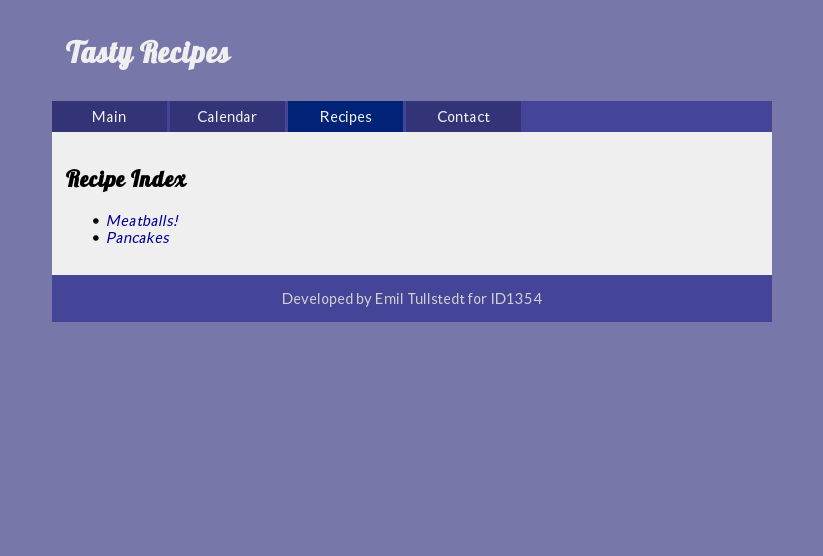
\includegraphics[scale=0.3]{noscript_recipe.png}
    \caption{Alternative navigation for JavaScript-less browsers}
    \label{fig:noscript}
  \end{center}
\end{figure}

To add the drop-down menus to the site, the first step would be to make sure that there are sensible alternatives for browser which has no JavaScript support. This was done by adding "navigation" pages that contains the same information that is in the drop-down menus. This can be seen in figure \ref{fig:noscript}.

Without any JavaScript loaded, these navigation sites are the target of the links that later will unfold a menu. To make sure the tags doesn't take you to another page when JavaScript is activated, this line of code executes on the relevant a-tags.
 
\begin{lstlisting}
function unregister_link(obj)
{
    $(obj).attr('href', '#');
}
\end{lstlisting}

This function should be run in another function we call \texttt{register\_dropdown}. The drop-down menu is an absolute positioned div with \texttt{a}-tags for every item. This dropdown is styled using:

\begin{lstlisting}
nav .dropdown                                                                   
{                                                                               
    display: none;                                                              
    position: absolute;                                                         
    left: 0;                                                                    
    top: 0;                                                                     
    z-index:100;                                                                
}                                                                               
                                                                                
nav .dropdown a                                                                 
{                                                                               
    background: #ee6666;                                                        
    display: block;                                                             
    clear: both;                                                                
    margin-top: 2px;                                                            
}  
\end{lstlisting}

You can note that the \texttt{left} and \texttt{top} are 0, which would imply that the drop-down menus are always positioned in the top left corner. This is further fixed in JavaScript by the code

\begin{lstlisting}
if ($(document).width() > 480) {                                    
	var button_offset  = $(object).offset();                        
	button_offset.top += $(object).height()+15;                     
	$(menu).css('left', button_offset.left);                        
	$(menu).css('top', button_offset.top);                          
}
\end{lstlisting}

The comparator is there to ensure that smaller screen resolutions works well, where media-queries makes the CSS of the drop-down menu for small screens equal to:

\begin{lstlisting}
nav .dropdown                                                               
{                                                                           
    display: none;                                                          
    position: relative;                                                     
}                                                                           
                                                                                
nav .dropdown.show                                                          
{                                                                           
    display: block;                                                         
}
\end{lstlisting}


\begin{figure}[!h]
  \begin{center}
    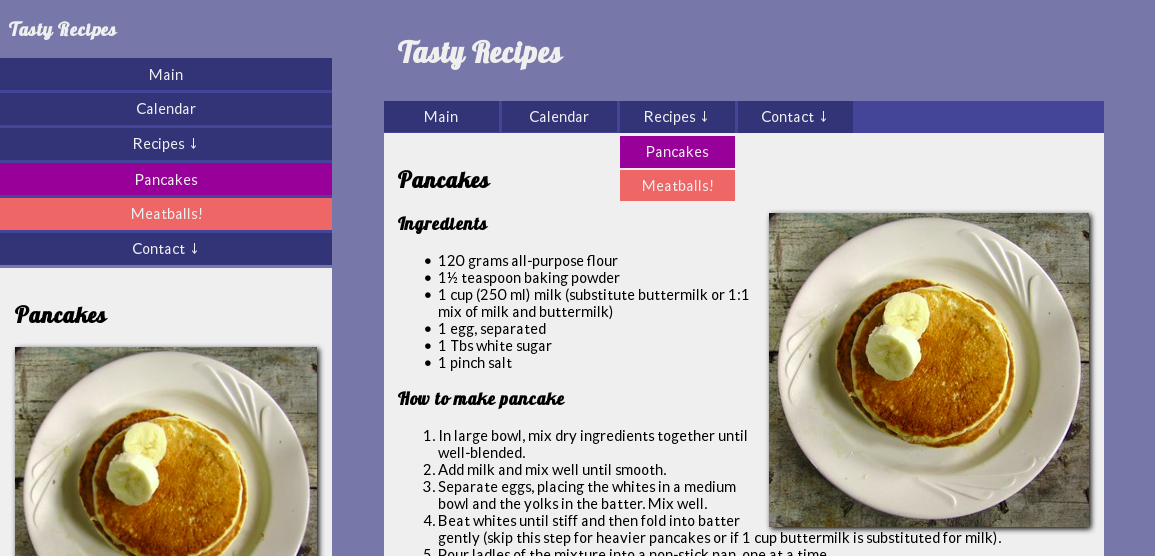
\includegraphics[scale=0.3]{dropdown_both.png}
    \caption{Side-by-side drop-down menu for larger and smaller screens}
    \label{fig:dropdown}
  \end{center}
\end{figure}

The result of this can be seen in figure \ref{fig:dropdown}.

To ensure the modularity of the dropdown code, a JavaScript function to register an object as a drop-down menu was made. This function can be seen in it's entirety below:

\begin{lstlisting}
function register_dropdown(shortid)                                             
{                                                                               
    var object = "#nav_" + shortid;                                             
    var toggle_menu =                                                           
        function() {                                                            
            var menu = "#dropdown_" + shortid;                                  
                                                                                
            if($(menu).hasClass('show'))                                        
            {                                                                   
                $(menu).removeClass('show');                                    
                $(menu).fadeOut();                                              
                return;                                                         
            }                                                                   
                                                                                
            if ($(document).width() > 480) {                                    
                var button_offset  = $(object).offset();                        
                button_offset.top += $(object).height()+15;                     
                $(menu).css('left', button_offset.left);                        
                $(menu).css('top', button_offset.top);                          
            }                                                                   
                                                                                
            close_dropdowns();                                                  
            $(menu).addClass('show');                                           
            $(menu).fadeIn();                                                   
                                                                                
            setTimeout(function() { $(document).click(close_dropdowns); }, 15); 
        };                                                                      
                                                                                
    unregister_link(object);                                                    
    $(object).append(" \/");                                                     
    $(object).addClass("dropdown_head");                                        
    $(object).click(toggle_menu);                                               
}   
\end{lstlisting}

The most interesting part of this code is probably \texttt{\$(document).click(close\_dropdowns);} which registers the function close\_dropdowns to a click anywhere on the page. This makes the menu close whenever you press something that isn't a link.

The close\_dropdowns function is defined as

\begin{lstlisting}
function close_dropdowns()                                                      
{                                                                               
    $('.dropdown.show').each(                                                   
        function() {                                                            
            $(this).fadeOut(400, function() {                                   
                $(this).removeClass('show');                                    
                $(this).css('left', '0px');                                     
                $(this).css('top', '0px');                                      
        });                                                                     
    });                                                                         
                                                                                
    $(document).unbind('click');                                                
} 
\end{lstlisting}

which pretty much resets the drop-down menu to it's defaults.

\subsection{Comments}

\begin{figure}[!h]
  \begin{center}
    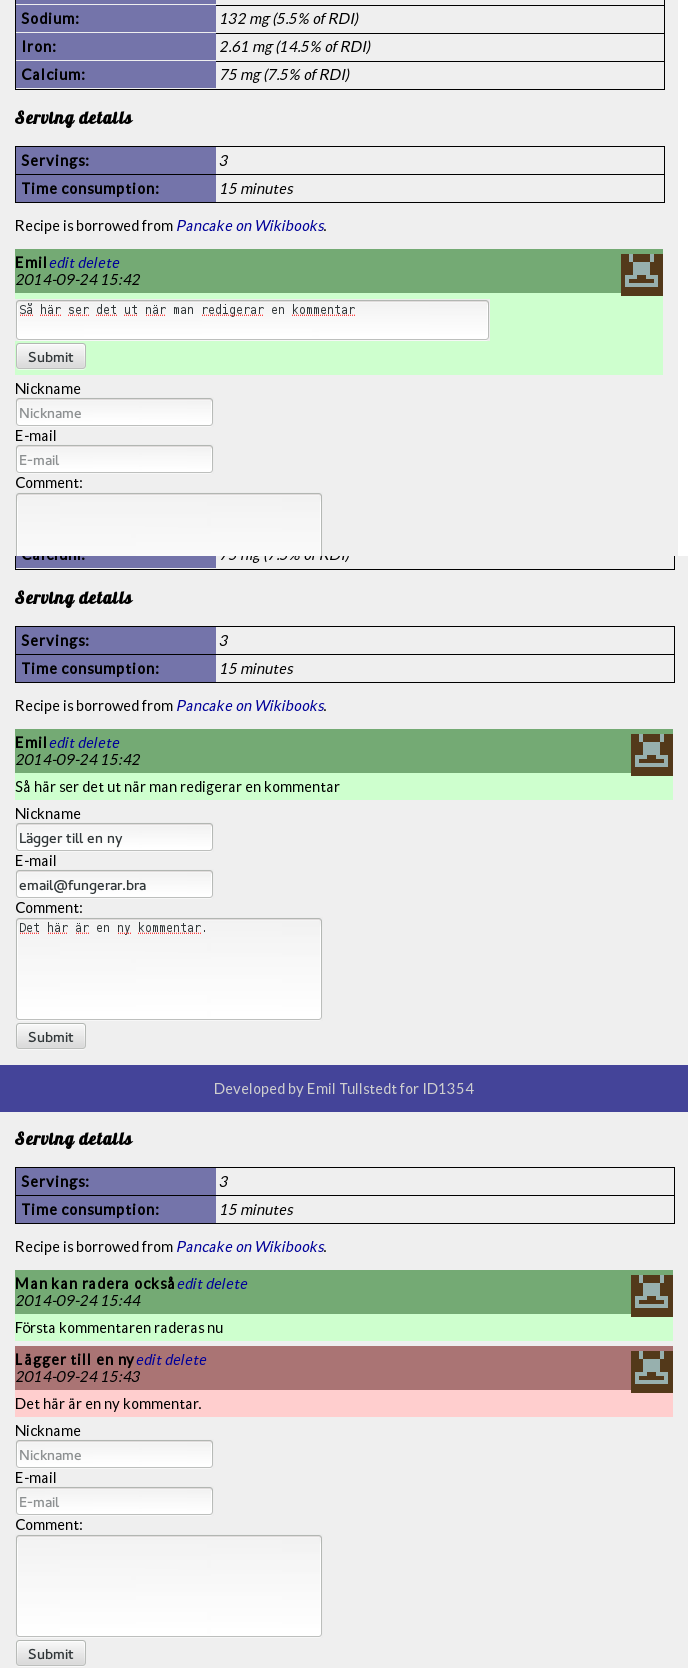
\includegraphics[scale=0.3]{kommentar_all.png}
    \caption{Editing, adding and deleting comments}
    \label{fig:comments}
  \end{center}
\end{figure}

The ability to make volatile comments is fulfilled by creating the comment-area with an input form. This input form is hijacked so that it doesn't send a \textit{POST/GET}-request on submit but rather creates a new DOM-object at the top of the comment area.

By inserting the code below into the function that takes care of new comments, the site ensured that all the fields was filled before the submit-action did anything.

\begin{lstlisting}                                                                         
            if (!name || !email || !comment) {
                e.preventDefault();
                return;                                              
            }
\end{lstlisting}

To delete a posted comment, it is as simple as binding the object-click to removing the comment. The \texttt{register\_delete\_comment} is fully written below:

\begin{lstlisting}
function register_delete_comment (button_class) {
    $(button_class).click(function (e) {
        var comment = $(this).closest('.comment');
        comment.remove();
        e.preventDefault();
    });
}    
\end{lstlisting}

To edit a comment, the value of the comment content is converted into a editable text area which is returned to a normal textbox when finished editing and submitting the form. This form is also hijacked to prevent unnecessary.
                
\subsection{Contact Us and About Us}

\begin{figure}[!h]
  \begin{center}
    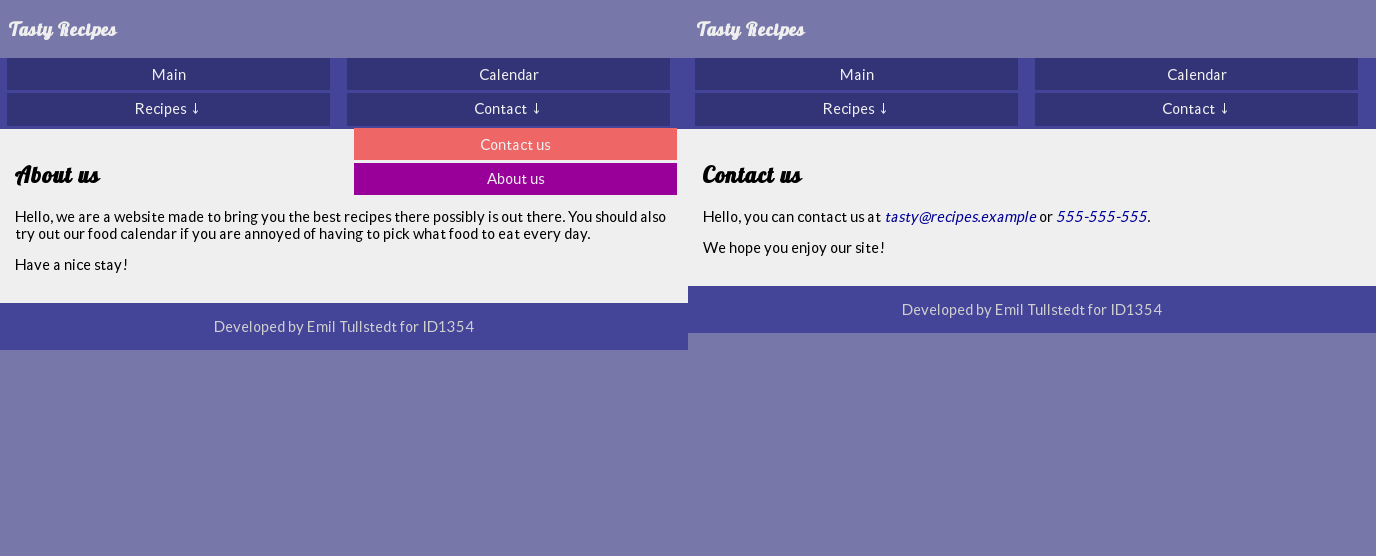
\includegraphics[scale=0.3]{contact_all.png}
    \caption{The contact }
    \label{fig:contact}
  \end{center}
\end{figure}

Simple contact us and about us was added to fulfill the requirements. These were simply modified versions of the front-page with different content. See figure \ref{fig:contact}.

\section{Discussion}

The addition of JavaScript felt quite unnecessary for this site. I would've preferred to use CSS to make the drop-down menu and to do the server side scripting before the JavaScript development is commenced. There are plenty of improvements that can be done to my version of the site, for example to structure everything more according the MVC. That was scrapped because of two reasons:

\begin{enumerate}
\item Adding more JavaScript libraries makes the site less stable
\item It was uncertain how the libraries would work together with the ambition of keeping the site non-dependent on JavaScript and CSS
\end{enumerate}

\end{document}
